\chapter{i numeri complessi}
%%%%%%%%%%%%%%%%%%%%%%%%
%%%%%%%%%%%%%%%%%%%%%%%%
%%%%%%%%%%%%%%%%%%%%%%%%
%%%%%%%%%%%%%%%%%%%%%%%%

Nel capitolo precedente abbiamo introdotto l'esponenziale complesso ed
abbiamo osservato che la funzione $f\colon \RR \to \CC$ definita da
$f(t) = e^{it}$ ha valori sulla circonferenza unitaria in quanto
$\abs{e^{it}}=1$. Tramite la definizione~\ref{def:sincos}
abbiamo introdotto le funzioni seno e coseno in
modo che risulti $f(t) = \cos t + i \sin t$.
Sappiamo che $f(0) = e^0 = 1$ e, per come abbiamo definito $\pi$,
sappiamo che $f(\pi/2) = i$.

\section{rappresentazione polare dei numeri complessi}

I numeri complessi di modulo uno vengono chiamati \emph{unitari}.
\mynote{complessi unitari}%
\index{complessi!unitari}%
\index{unitario}%
Geometricamente i numeri complessi unitari sono i punti della circonferenza
unitaria centrata nell'origine del piano complesso.
Se $z=x+iy$ è unitario si ha $x^2+y^2=1$.
I prodotti e i
reciproci dei numeri complessi unitari sono anch'essi unitari,
risulta quindi che tali numeri formano un \emph{sottogruppo moltiplicativo}%
\footnote{
Un \emph{gruppo} è un insieme su cui è definita una operazione
(spesso denotata con il simbolo della moltiplicazione) che sia associativa,
che abbia elemento neutro e tale che ogni elemento abbia un inverso.
}
del gruppo dei numeri complessi.

Ogni numero complesso $z$ potrà essere scritto nella forma
\[
  z = \rho \cdot u
\]
con $\rho\in \RR$, $\rho>0$ e $u\in\CC$ unitario.
Basta infatti
definire $\rho = \abs{z}$ e $u = z / \abs{z}$ (se $z\neq 0$, altrimenti
si potrà scegliere arbitrariamente $u=1$).

\begin{theorem}[argomento]
Sia $z\in \CC$ un numero complesso non nullo. Allora esiste un
unico $\theta\in [0,2\pi)$ tale che
\[
z = \abs{z} e^{i\theta}.
\]
Denoteremo tale valore di $\theta$ come l'\myemph{argomento} di $z$
e scriveremo
\[
  \theta = \arg z.
\]
Se $z=0$ porremo per convenzione $\arg z=0$.
\end{theorem}
%
\begin{proof}
Sia $z\in \CC$, $z\neq 0$ e poniamo $u = z/\abs{z}$.
Posto $u=x+iy$ con $x,y\in \RR$ si ha $\abs{u}^2 = x^2+y^2=1$.

Se $y\ge 0$ se vogliamo che $y=\sin \theta$ con $\theta\in [0,2\pi)$
dovrà necessariamente essere $\theta \in [0,\pi]$
(altrimenti si avrebbe $\sin \theta<0$).
E se vogliamo che sia $x=\cos \theta$ basterà (e si dovrà) scegliere
$\theta = \arccos x$.
Visto che $\sin^2 \theta + \cos^2\theta = 1 = x^2 + y^2$
sapendo che $\cos \theta = x$
si avrà
$\sin^2 \theta = y^2$ cioè $\abs{\sin \theta}=\abs y$.
Ma visto che $y\ge 0$ e $\sin \theta\ge 0$
avremo, come voluto, $\sin \theta = y$.
Se $y<0$ poniamo $\theta = 2\pi - \arccos x$
cosicché si avrà $\theta \in (\pi, 2\pi)$
e, come prima (verificare!),
$x=\cos \theta$, $y=\sin \theta$.

In ogni caso per ogni $z\neq 0$ abbiamo quindi trovato l'unico
$\theta\in [0,2\pi)$ tale che
\[
  u
  = x + i y
  = \cos \theta + i\sin \theta)
  = e^{i\theta}.
\]
da cui
\[
  z = \abs{z}\cdot e^{i\theta}.
\]
\end{proof}

Per ogni $z\in \CC$ posto
\[
  \rho = \abs{z}, \qquad \theta = \arg z
\]
si avrà quindi la \emph{rappresentazione esponenziale} o \emph{polare}
\[
  z = \rho e^{i\theta} = \rho \cdot \enclose{\cos \theta
  + i \sin \theta}.
\]
Se $z=x+iy$ è la \emph{rappresentazione cartesiana}, si avranno
le seguenti formule di conversione:
\[
\begin{cases}
  x = \rho \cos \theta\\
  y = \rho \sin \theta
\end{cases}
\qquad
\begin{cases}
 \rho = \sqrt{x^2+y^2}\\
 \theta = \arg z
\end{cases}
\]
con
\[
  \arg z =
  \begin{cases}
%   \arctg \frac y x & \text{se $x>0$,} \\
   \frac \pi 2 - \arctg \frac x y & \text{se $y>0$,} \\
   \frac 3 2 \pi- \arctg \frac x y & \text{se $y<0$,} \\
   \pi & \text{se $y=0$ e $x<0$,} \\
   0 & \text{se $y=0$ e $x\ge 0$.}
   \end{cases}
\]

\section{interpretazione geometrica}
\label{sec:radianti}

Vogliamo ora interpretare geometricamente $\theta = \arg z$ come la misura
di un angolo. Per fare ciò dobbiamo però capire cosa si intende per angolo
e come si misura un angolo.
In questa sezione ragioneremo in maniera intuitiva in quanto le proprietà
formali analitiche delle operazioni sui numeri complessi
sono già state determinate e quello
che vogliamo fare è darne una interpretazione geometrica.
Daremo quindi per scontate le proprietà geometriche del piano euclideo.

Un \emph{angolo},
geometricamente, è la regione piana delimitata da due semirette
uscenti da uno stesso punto. Le due semirette si chiamano \emph{lati}
dell'angolo e il punto in comune si chiama \emph{vertice}.

Due angoli $\alpha,\beta$ si dicono congruenti se è possibile traslare e ruotare uno dei
due angoli (diciamo $\alpha$) in modo che si sovrapponga all'altro.
In particolare sarà sempre possibile trovare una traslazione
che manda il vertice dell'angolo $\alpha$ sul vertice dell'angolo $\beta$
e sarà possibile trovare una rotazione che fa coincidere uno dei due lati
in modo che uno dei due angoli copra interamente l'altro.
Sia $\alpha'$ la roto-traslazione di $\alpha$ così individuata.
Se $\alpha'=\beta$ diremo che i due angoli sono congruenti,
altrimenti se
$\alpha' \supset \beta$ diremo che $\alpha$ è maggiore di $\beta$ e se
invece $\alpha' \subset \beta$ diremo che $\alpha$ è minore di $\beta$.
Con un procedimento simile è in genere possibile sommare due angoli:
si sposta uno dei due tramite una roto-traslazione in modo da far coincidere
il vertice e un lato dei due angoli e in modo
che i due angoli non si sovrappongano
(questo non è sempre possibile perché se gli angoli sono troppo grandi
si sovrapporranno sempre).
La loro unione sarà un angolo
che chiamiamo somma degli angoli dati.

Misurare un angolo significa associare ad ogni angolo un numero (reale positivo)
in modo che
si abbiano le seguenti proprietà: angoli congruenti hanno la stessa misura,
angoli maggiori hanno misure maggiori (proprietà di monotonia)
e la misura della somma di due angoli è la somma delle misure
(additività).
Si può intuire che una volta scelto quale angolo ha misura $1$
(l'unità di misura) la misura di ogni altro angolo sarà univocamente determinata
da queste proprietà. Infatti la misura dei multipli e dei sottomultipli
dell'unità è determinata dalla additività della misura e la misura
degli angoli incommensurabili si potrà ottenere per approssimazione
sfruttando la monotonia.

Se ora identifichiamo il piano euclideo con il piano complesso ogni angolo
potrà essere traslato e ruotato in modo che uno dei due lati vada
a coincidere con la semiretta dei reali positivi e in modo che l'angolo si
estenda al di sopra di tale semiretta e sia delimitato da una seconda
semiretta passante per un punto $u$ a distanza $1$ dall'origine
ovvero con $\abs{u}=1$. Vogliamo giustificare il fatto che $\theta = \arg u$
può essere scelto come misura dell'angolo.
Studiando la monotonia delle funzioni $\cos$ e $\sin$ si può verificare facilmente
che $\theta$ è crescente con l'angolo. Più rilevante è chiedersi se
$\theta$ è additivo.
Siano $u,v\in \CC$ due numeri complessi unitari che rappresentino due diversi
angoli. Sia $\theta = \arg u$ e $\phi=\arg v$ da cui
$u=e^{i\theta}$ e $v=e^{i\phi}$.
Consideriamo la trasformazione $R_\theta(z) = e^{i\theta}\cdot z$.
Si nota che $R_\theta$ è una trasformazione rigida del piano ovvero
una trasformazione che mantiene la distanza tra i punti
(una \emph{isometria})
in quanto essendo $\abs{e^{i\theta}}=1$ si ha
\[
\abs{R_\theta(z)-R_\theta(w)} = \abs{e^{i\theta}z-e^{i\theta}w}
= \abs{e^{i\theta}}\cdot\abs{z-w} = \abs{z-w}.
\]
Inoltre $R_\theta(0)=0$ e $R_\theta(1)=u$ significa che $R_\theta$ non è altro che una
rotazione che tiene fissa l'origine e manda la semiretta dei reali
positivi nella semiretta uscente da $0$ e passante per $u=e^{i\theta}$.
Dunque $R_\theta$ è la trasformazione che rende l'angolo identificato
dal numero complesso unitario $v$ in un angolo adiacente a quello
identificato da $u$. Quindi la somma (geometrica) degli angoli
$u$ e $v$ è identificata dal numero complesso unitario
$R_\theta(v) = u\cdot v$.
Ma, per la proprietà additiva dell'esponenziale complesso,
\[
 u\cdot v = e^{i\theta} \cdot e^{i\phi} = e^{i(\theta+\phi)}
\]
e dunque se $\theta+\phi<2\pi$ si ha
\[
 \arg(u\cdot v) = \theta + \phi = \arg(u) + \arg(v)
\]
che corrisponde alla proprietà additiva della misura degli angoli.

L'angolo unitario identificato dal numero complesso $e^i$
si chiama \myemph{radiante} ed è l'unità di misura che abbiamo scelto
per gli angoli.
L'angolo retto sarà identificato dal numero complesso $i=e^{i\frac \pi 2}$
e avrà una misura pari a $\frac \pi 2$ radianti. L'angolo piatto sarà identificato
dal numero complesso $-1 = e^{i\pi}$ e avrà una misura di $\pi$ radianti.
Geometricamente la misura degli angoli può essere data dalla lunghezza
dell'arco di raggio unitario identificato dall'angolo. Dunque la definizione
geometrica di $\pi$ (rapporto tra lunghezza della circonferenza e diametro)
corrisponde a richiedere che la semicirconferenza unitaria abbia misura
$\pi$ radianti.
Questo significa che la definizione analitica di $\pi$ che abbiamo
dato (teorema~\ref{th:pi}) si riconcilia con la definizione geometrica.

Possiamo riconciliare definizione analitica e geometrica di $\pi$ anche
con delle osservazioni dirette.

\begin{remark}[lunghezza della circonferenza tramite moto circolare uniforme]
Si considera la curva $t\mapsto e^{it}$
come l'equazione oraria del moto di un punto
che si muove nel piano complesso. Visto che $\abs{e^{it}}=1$
tale punto si muove sulla circonferenza unitaria.
Possiamo determinare la velocità istantanea del punto considerando
la variazione della posizione:
\[
  \frac{e^{i(t+\Delta t)}-e^{it}}{\Delta t}
  = e^{it}\cdot \frac{e^{i\Delta t}-1}{\Delta t}.
\]
Prendendo un incremento temporale $\Delta t = \eps /n$ con $n\to +\infty$
si osserva che il modulo della velocità è dato da
\[
 v = \lim_{n\to +\infty} \abs{e^{it}}\cdot \abs{\frac{e^{i\frac \eps n}-1}{\frac \eps n}}
\]
e visto che $\abs{e^{it}}=1$ ricordando il limite notevole~\eqref{eq:limite_exp_complesso}
(teorema~\ref{th:exp_complesso}) si ottiene che la velocità è pari ad $1$.
Significa che il punto $e^{it}$ si muove sulla circonferenza unitaria
con velocità unitaria e quindi la lunghezza della curva percorsa risulta
numericamente uguale al tempo trascorso.
Visto che per $t$ che varia da $0$ a $2\pi$
il punto compie un giro completo attorno alla circonferenza unitaria
significa che la lunghezza della circonferenza unitaria è $2\pi$.
\end{remark}

\begin{remark}[lunghezza della circonferenza tramite approssimazione con poligonali]
\label{rem:pi}
Possiamo
calcolare la lunghezza della circonferenza unitaria come il limite dei perimetri dei poligoni
di $N$ lati iscritti nella circonferenza.
Fissato $N$
consideriamo per $k=0, \dots, N$ i punti
\[
  u_k = e^{i\frac{2\pi k}{N}}.
\]
Osserviamo che
\[
  \abs{u_{k+1}-u_k}
  = \abs{e^{i\frac{2\pi (k+1)} N}-e^{i\frac{2\pi k} N}}
  = \abs{e^{i\frac{2\pi k}{N}}} \cdot \abs{e^{i\frac{2\pi}{N}}-1}
  = \abs{e^{i\frac{2\pi}{N}}-1}
\]
cioè i punti $u_k$ sono equidistanti tra loro.
Si noti che $u_0=u_N=1$
e quindi i punti $u_1,\dots, u_N$ sono gli $N$ vertici
di un poligono regolare di $N$ lati iscritto nella
circonferenza unitaria. Il perimetro del poligono è quindi
dato da
\[
P_N = N \cdot \abs{e^{i\frac{2\pi}{N}}-1}
\]
e per $N\to +\infty$ si ha,
sempre utilizzando il limite notevole~\eqref{eq:limite_exp_complesso}
\[
P_N = 2 \pi \cdot \abs{\frac{e^{i\frac{2\pi}{N}}-1}{\frac{2\pi}{N}}}
  \to 2\pi.
\]
\end{remark}

\begin{remark}[matrici di rotazione]
Fissato $\theta\in \RR$
consideriamo, come prima, la funzione $R_\theta\colon \CC \to \CC$,
$R_\theta(z) = e^{i\theta}\cdot z$.
Un altro modo per convincerci che $R_\theta$
rappresenta una rotazione di $\theta$ radianti è
quello di guardare la matrice associata.
Se identifichiamo il piano complesso $\CC$ con $\RR^2$ la trasformazione
$R_\theta$ può essere rappresentata
da una matrice $M_\alpha$ che ha come
colonne le coordinate di $R_\theta(1) = e^{i\theta} = \cos \theta + i \sin \theta$
e le coordinate di $R_\theta(i) = e^{i\theta}\cdot i = -\sin \theta + i \cos \theta$:
\[
  M_\alpha =
  \begin{pmatrix}
  \cos \alpha & -\sin \alpha \\
  \sin \alpha & \cos \alpha
  \end{pmatrix}.
\]
\end{remark}

\begin{remark}[interpretazione geometrica del prodotto di numeri complessi]
Possiamo ora dare una interpretazione geometrica del prodotto tra
due numeri complessi $z,w\in \CC$.
Se $z\neq 0$ possiamo scrivere $z = \abs{z} \cdot e^{i\theta}$
con $\theta= \arg z$, cosicché:
\[
  z \cdot w = \abs{z} \cdot R_\theta(w).
\]
Si capisce quindi che il numero complesso $z\cdot w$ si ottiene ruotando
$w$ dell'angolo identificato da $z$ con l'asse dei reali positivi, e quindi
riscalando il punto ottenuto di un fattore $\abs{z}$.
Se poniamo $\psi = \arg w$ possiamo interpretare la moltiplicazione complessa
in coordinate polari:
\[
  z \cdot w = \abs{z}e^{i\theta}\cdot \abs{w} e^{i\psi}
   = \abs{z} \cdot \abs{w} \cdot e^{i(\theta + \phi)}.
\]
Dunque il prodotto di due numeri complessi è quel numero complesso
che ha come modulo il prodotto dei moduli e come argomento
la somma (a meno di multipli di $2\pi$) degli argomenti.
\end{remark}


\begin{remark}[interpretazione geometrica dell'esponenziale complesso]
Ricordiamo che (teorema~\ref{th:exp_exp})
\[
  e^{iy} = \lim_{n\to +\infty} \enclose{1+\frac{iy}{n}}^n.
\]

Possiamo osservare che se $y\in \RR$
i punti $(1+iy/n)^k$ per $k=1\dots n$
sono i vertici di una spezzata
formata da $n$ segmenti
di lunghezza
\begin{align*}
 \abs{\enclose{1+\frac{iy}n}^{k+1}\!\!\! - \enclose{1+ \frac{iy}n}^k}
 &= \abs{\enclose{1+\frac{iy}n}^k\cdot \enclose{1+\frac{iy}n -1}}\\
 &= \enclose{\sqrt{1+\frac{y^2}{n^2}}}^{\!\!k} \cdot \frac{\abs y}{n}
 \le \enclose{1+\frac{y^2}{n^2}}^{\frac n 2}\cdot \frac{\abs{y}}{n}.
\end{align*}
In particolare la lunghezza totale della spezzata $\ell_n$ può essere stimata
come segue
\[
  \abs{y}
  \le \ell_n
  \le \enclose{1+\frac{y^2}{n^2}}^{\frac n 2} \cdot \abs{y}
\]
da cui osservando che
\[
 \enclose{1+\frac{y^2}{n^2}}^{\frac n 2} \to 1
\]
e utilizzando il criterio del confronto
si ottiene $\ell_n \to \abs{y}$.

Si osserva anche che i punti di tale spezzata si avvicinano
sempre di più alla circonferenza unitaria, infatti:
\[
  1
  \le \abs{\enclose{1 + \frac i n}^k}
  \le \abs{1+\frac i n}^n
  = \enclose{1 + \frac 1 {n^2}}^{\frac n 2}
  \to 1.
\]

E' dunque sensato pensare che il punto $e^{iy}$ sia il punto
della circonferenza unitaria che identifica un arco di lunghezza $\abs y$
a partire dal punto $1$ sull'asse reale.
Se $y>0$ l'arco è misurato in senso antiorario, altrimenti in senso orario.
Avremo dunque $\arg\enclose{e^{iy}} = y$ essendo $y$ la lunghezza dell'arco
ovvero la misura in radianti dell'angolo corrispondente.
\end{remark}

\section{radici complesse $n$-esime}

Sia $c\in \CC$ un numero
complesso $c\neq 0$.
Ci poniamo il problema di determinare le soluzioni complesse
dell'equazione
\[
  z^n = c.
\]
Tali soluzioni saranno chiamate \myemph{radici $n$-esime} di $c$.

Scriviamo $c$ e $z$ in forma esponenziale:
\[
  c = r e^{i\alpha}, \qquad
  z = \rho e^{i\theta}.
\]
Si avrà allora
\[
  z^n = \rho^n (e^{i\theta})^n = \rho^n e^{i n \theta}.
\]
Affinche sia $z^n = c$ si dovrà avere l'uguaglianza dei moduli, cioè $\rho^n = r$ e l'uguaglianza a meno di multipli interi di $2\pi$ degli argomenti:
$n \theta = \alpha + 2 k \pi$ con $k\in \ZZ$.
Dunque si trova
\[
  \theta = \frac{\alpha}{n} + k\frac{2\pi}{n}
\qquad k \in \ZZ.
\]
Osserviamo ora che per $k=0,\dots, n-1$ il secondo addendo
$k 2\pi /n$ assume $n$ valori distinti compresi in $[0,2\pi)$.
Per gli altri valori di $k$ si ottengono degli angoli che differiscono
da questi di un multiplo di $2\pi$ e quindi non si trovano
altre soluzioni.

Dunque l'equazione $z^n = c$ per $c\neq 0$ ha $n$ soluzioni distinte date
da
\[
z_k = \sqrt[n]{r} \cdot e^{i\alpha/n + 2k\pi i /n},
\qquad k=0,1, \dots, n-1
\]
dove $\alpha = \arg(c)$ e $r = \abs{c}$.
Dal punto di vista geometrico si osserva che
$z_0$ è il numero complesso con modulo la radice $n$-esima del numero
dato $c$ e argomento pari ad un $n$-esimo dell'argomento di $c$.
Tutte le altre soluzioni si trovano sulla circonferenza centrata in $0$
e passante per $z_0$ e risultano essere, insieme ad $z_0$, i vertici
di un $n$-agono regolare.

In particolare nel caso $c=1$ si osserva che le radici $n$-esime dell'unità
si rappresentano geometricamente come i vertici dell'$n$-agono regolare iscritto
nella circonferenza unitaria e con un vertice in $z_0=1$.

\begin{exercise}
Si trovino le soluzioni $z \in \CC$ delle seguenti equazioni.
Scrivere le soluzioni in forma polare e cartesiana.
\begin{gather*}
   z^4 = -4 \\
   z^6 = i\\
   z^3 = -8i \\
   z^4 = z\\
   z^2 + 1 = i\sqrt{3} \\
   (z-i)^4 = 1\\
   1 + z + z^2 + z^3 = 0\\
   z^{14} - z^6 - z^8 + 1 = 0
\end{gather*}
\end{exercise}

\section{polinomi}

Se $\KK$ è un campo\footnote{%
Ma più in generale è sufficiente
avere un \emph{anello}: un insieme su cui sono definite le operazioni
di somma e prodotto come su un campo ma su cui non si richiede
l'esistenza dell'inverso moltiplicativo.
E' abbastanza comune, ad esempio, considerare polinomi
a coefficienti interi.}
(a noi interessa in particolare $\KK=\RR$ o $\KK=\CC$)
possiamo considerare tutte le espressioni
(formalmente: alberi di valutazione)
che possono essere costruite utilizzando le operazioni
di somma e prodotto a partire da coefficienti presi da $\KK$
e una variabile che possiamo chiamare $x$.
Queste verranno chiamate \emph{espressioni polinomiali} su $\KK$
(o a coefficienti in $\KK$)
nella variabile $x$. Un esempio di espressione polinomiale
nella variabile $x$ a coefficienti in $\RR$ può essere:
\[
  P(x) = \enclose{\frac 1 2 x+\sqrt 3}\cdot(x\cdot (2+x) + 3\cdot(-1+x))
\]
ovvero l'albero di valutazione:
\begin{center}
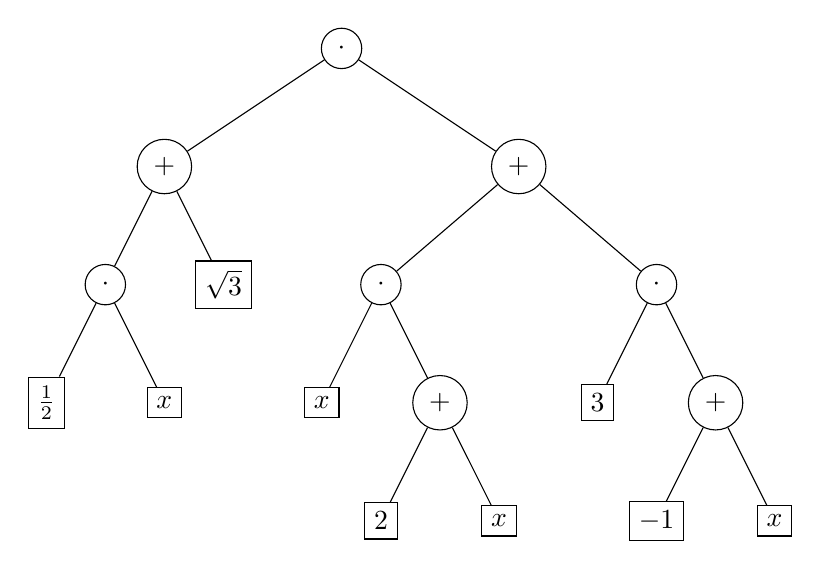
\begin{tikzpicture}
\node [circle,draw] {$\cdot$}
  child {
    node [circle,draw,xshift=-15mm] {$+$}
    child {
      node [circle,draw] {$\cdot$}
      child {node [draw]{$\frac 1 2$}}
      child {node [draw]{$x$}}
    }
    child {node [draw] {$\sqrt 3$}}
  }
  child {
    node [circle,draw,xshift=15mm] (M) {$+$}
    child {
      node [circle,draw,xshift=-10mm]{$\cdot$}
      child {node [draw]{$x$}}
      child {
        node [circle,draw]{$+$}
        child {node [draw] {$2$}}
        child {node [draw] {$x$}}
        }
      }
    child {
      node [circle,draw,xshift=10mm]{$\cdot$}
      child {node [draw] {$3$}}
      child {
        node [circle,draw] {$+$}
        child {node [draw] {$-1$}}
        child {node [draw] {$x$}}
        }
    }
  };
\end{tikzpicture}
\end{center}
Sviluppando tutti i prodotti tramite la proprietà distributiva,
ogni espressione di questo tipo può essere ricondotta ad una
somma di prodotti di costanti per potenze intere della variabile
$x$:
\begin{align*}
P &= \enclose{\frac 1 2 x+\sqrt 3}\cdot(x\cdot (2 + x)
+ 3\cdot(-1+x))\\
&= \enclose{\frac 1 2 x + \sqrt 3} (2x+x^2-3+3x) \\
&= - 3 \sqrt 3 + \enclose{-\frac{3}{2}+ 5\sqrt 3} x
  + \enclose{\frac{5}{2}+\sqrt 3} x^2 + \frac 1 2 x^3.
\end{align*}
Si ottiene quindi un polinomio in \emph{forma canonica}
\[
  P = a_0 + a_1 x + a_2 x^2 + \dots + a_n x^n
       = \sum_{k=0}^n a_k x^k.
\]
Due espressioni polinomiali che hanno la stessa
forma canonica si diranno equivalenti: diremo
allora che rappresentano lo stesso \myemph{polinomio}.
Nella forma canonica si intende che siano presenti tutte
le potenze di $x$ da $x^0 = 1$, $x^1=x$ \dots fino ad
una potenza massima $x^n$.
Se una potenza non compare
nell'espressione si può comunque inserire mettendo
il coefficiente corrispondente uguale a zero.
La potenza massima, invece, dovrà avere un coefficiente
diverso da zero, altrimenti si dovrà decrementare
$n$ finché non si giunge a tale proprietà.
Tale esponente $n$ si chiama \myemph{grado del polinomio}
che denoteremo con $\deg P$.
Se la potenza massima è $0$ avremo un unico coefficiente
$a_0$. In tal caso il grado del polinomio è nullo (zero)
e diremo che il polinomio è \emph{costante}.
Se tutti i coefficienti sono nulli (uguali a zero)
avremo formalmente
una somma vuota, diremo che il polinomio è nullo e,
per convenzione, porremo $\deg P = -\infty$.

Se $\KK$ è un campo denoteremo con $\KK[x]$ l'insieme
di tutti i polinomi con coefficienti in $\KK$ e variabile $x$.
Si tratta quindi di espressioni polinomiali identificate
a meno di equivalenza. Ogni polinomio è univocamente
determinato dalla sua forma canonica ovvero dall'avere
un grado $n \in \NN \cup \{-\infty\}$ e una lista
di $n+1$ coefficienti:
\[
  (a_0, \dots, a_n) \in \KK^{n+1}
\]
(una lista vuota nel caso $n=-\infty$).
I polinomi possono essere sommati tra di loro
e moltiplicati per qualunque elemento $\KK$ del campo
e formano dunque uno spazio vettoriale
sul campo $\KK$. Inoltre è possibile moltiplicare
tra loro due polinomi (si parla in questo
caso di $\KK$-algebra).

Più esplicitamente se $P$ e $Q$ sono polinomi
scritti in forma canonica:
\[
  P = \sum_{k=0}^n a_k x^k, \qquad Q = \sum_{k=0}^m b_k x^k
\]
si avrà:
\[
  P + Q = \sum_{k=0}^{\max\{n,m\}} (a_k+b_k) \cdot x^k
\]
dove si intende che $a_k=0$ per $k>n$ e $b_k=0$ per $k>m$.
Si osserva quindi che il grado della somma di due polinomi
è minore o uguale alla somma dei gradi dei due polinomi.
Se $t\in \KK$ avremo:
\[
  t P = \sum_{k=0}^n (ta_k)\cdot x^k.
\]
Per quanto riguarda il prodotto si avrà invece:
\begin{align*}
  P\cdot Q
  &= \enclose{\sum_{k=0}^n a_k x^k}\cdot \enclose{\sum_{j=0}^n b_j x^j}
  = \enclose{\sum_{k=0}^n a_k \enclose{\sum_{j=0}^m a_j x^j} x^k} \\
  &= \enclose{\sum_{k=0}^n \sum_{j=0}^m a_k a_j x^{j+k}}
  = \sum_{s=0}^{m+n} \enclose{\sum_{j=0}^s a_j b_{s-j}} x^s.
\end{align*}
Dunque si osserva che il grado del prodotto è uguale
alla somma dei gradi.

Ogni polinomio in forma canonica è scritto come
combinazione lineare dei \emph{monomi} $x^k$:
significa che una base dello spazio vettoriale $\KK[x]$ è data dai
polinomi
\[
  1, x, x^2, x^3, \dots, x^n, \dots
\]
Dunque $\KK[x]$ è uno spazio vettoriale di dimensione
infinita. Fissato $n\in \NN$ possiamo considerare
il sottoinsieme di $\KK[x]$ formato da tutti
i polinomi di grado inferiore a $n$. E' chiaro
che tale insieme è in realtà un sottospazio vettoriale
di $\KK[x]$ di dimensione $n$ e una base di tale
sottospazio è dato dai monomi:
\[
  1, x, x^2, \dots, x^{n-1}.
\]

\begin{theorem}[divisione di Euclide]
\label{th:divisione_polinomi}%
\index{divisione tra polinomi}%
\index{polinomio!divisione}%
\index{polinomio!algoritmo di Euclide}%
\index{Euclide!algoritmo di divisione}%
\index{algoritmo!di Euclide}%
Dati due polinomi $P$ e $S\neq 0$ in $\KK[x]$ è possibile
trovare, in modo unico, due polinomi $Q$ (quoziente)
e $R$ (resto) in $\KK[x]$ con $\deg R < \deg R$
tali che:
\[
  P = Q \cdot S + R.
\]
\end{theorem}
%
\begin{proof}
\emph{Passo 1:} supponiamo che sia $\deg P < \deg S$.
In questo caso deve necessariamente essere $Q=0$ altrimenti
si avrebbe $\deg (Q\cdot S) = \deg Q + \deg S \ge \deg S > \deg R$ da cui
$\deg (Q\cdot S + R) = \deg(Q\cdot S) = \deg Q + \deg S > \deg P$
e non si potrebbe avere l'uguaglianza $P = Q\cdot S + R$.
Ma posto $Q=0$ e $R=P$ si ha $\deg R = \deg P < \deg S$
e l'uguaglianza è certamente (e unicamente) soddisfatta.

\emph{Passo 2:} supponiamo che sia $\deg P \ge \deg S$.
Poniamo $N=\deg P$ e $M=\deg S$.
Sia $a_N\neq 0$ il coefficiente del termine di grado massimo
di $P$ e $b_M\neq 0$ il coefficiente di grado massimo
del polinomio $S$.
E' allora facile verificare che il polinomio
\[
\frac{a_N}{b_M} \cdot x^{N-M}\cdot S
\]
ha lo stesso grado di $P$ e il suo coefficiente di grado
massimo è uguale ad $a_N$ in quanto è il prodotto di
$a_N/b_M$ per $b_M$.
Dunque il polinomio
\[
 P_1 = P - \frac{a_N}{b_N} \cdot x^{N-M}\cdot S
\]
ha grado strettamente inferiore a $P$.
Possiamo ora supporre, mediante un ragionamento induttivo
su $\deg P - \deg S$
che per il polinomio $P_1$ il risultato del teorema sia
valido cioè
che esistano, unici, dei polinomio $Q_1$ e $R$
con $\deg R < \deg S$ tali che
\[
  P_1 = Q_1 \cdot S + R.
\]
Il caso base del ragionamento induttivo,
$\deg P = \deg S$, è garantito dal Passo 1.
Avremo allora:
\begin{align*}
  P &= P_1 + \frac{a_N}{b_N} x^{N-M}\cdot S\\
    &= Q_1 \cdot S + R_1 + \frac{a_N}{b_N} x^{N-M}\cdot S\\
    &= (\frac{a_N}{b_N} x^{N-M} + Q_1) \cdot S + R_1.
\end{align*}
Posto quindi
\[
 Q = \frac{a_N}{b_N} x^{N-M} + Q_1
\]
il risultato è dimostrato.
\end{proof}

La dimostrazione del teorema precedente fornisce anche un
algoritmo, chiamato \emph{algoritmo di Euclide},
per eseguire la divisione (con resto) tra polinomi.
Lo sperimentiamo nel seguente esercizio.

\begin{exercise}
Sia $P = x^4-3 x^2 + 2x + 1$ e $S = x^2-1$.
Eseguire la divisione con resto cioè:
trovare $Q$ ed $R$ con $\deg R < \deg S$ tali che
\[
P = Q \cdot S + R.
\]
\end{exercise}
%
\begin{proof}[Svolgimento.]
Il rapporto tra i termini di grado massimo di
$P$ e $S$ è $x^4/x^2 = x^2$.
Dunque consideriamo come primo monomio $x^2$.
Si ha
\begin{align*}
  P_1
  &= P - x^2 \cdot S
  = x^4-3x^2+2x+1 - x^4+x^2 \\
  &= -2x^2+2x+1.
\end{align*}
Ripetiamo il procedimento con $P_1$ al posto di $P$.
Il rapporto tra i termini di grado massimo di $P_1$ e $S$
è il monomio $-2$. Si ha
\[
  P_2 = P_1 - (-2) S = -2x^2 + 2x + 1 + 2x^2 - 2 = 2x -1.
\]
Visto che $\deg P_2 < \deg S$ la divisione termina e
si pone $R = 2z-1$.
Si ha quindi $Q = x^2 - 2$ (la somma dei monomi trovati)
e risulta:
\[
  P = (x^2 - 2)\cdot S + 2x -1.
\]
\end{proof}

Dato un polinomio $P\in \KK[x]$ e un numero $a\in \KK$
è possibile prendere l'espressione rappresentata da
$P$ e sostiture alla variabile $x$ il valore $a$.
E' chiaro allora che svolgendo le operazioni di somma
e moltiplicazione si ottiene un valore in $\KK$
che denoteremo con $P(a)$.
Ogni polinomio $P\in \KK[x]$ identifica quindi una funzione
$P\colon \KK \to \KK$, $x\mapsto P(x)$ che chiameremo
\emph{funzione polinomiale} associata a $P$.

\begin{theorem}[Ruffini]
\label{th:Ruffini}%
\index{teorema!di Ruffini}%
\index{Ruffini}%
Sia $P\in \KK[x]$ un polinomio non nullo.
Se $x_0 \in \KK$ è tale che $P(z_0)=0$
allora esiste un polinomio $Q$ con $\deg Q = (\deg P) - 1$
tale che
\[
  P = (x-x_0)\cdot Q.
\]
\end{theorem}
%
\begin{proof}
In base al teorema precedente si può fare la divisione tra
$P$ e $S = x - x_0$ per ottenere un polinomio $Q$ e un resto
$R$ con $\deg r < 1$ tali che
\[
  P = (x-x_0)\cdot Q + R.
\]
Siccome $\deg R < 1$ si ha in effetti che $R=c\in \KK$
è un polinomio costante e dunque
\[
  P = (x-x_0) \cdot Q + c
\]
ma valutando $P$ in $x=x_0$ si scopre che
\[
 P(x_0) = 0\cdot Q(x_0) + c = c
\]
dunque $c=P(x_0) = 0$.
\end{proof}

Possiamo ora chiederci se polinomi diversi corrispondono
a funzioni polinomiali diverse.
In generale questo non è vero, se ad esempio prendessimo
come campo $\KK=\ZZ_2 = \{0,1\}$, un campo finito
in cui $1+1=0$ scopriremmo che la funzione polinomiale
$P(x) = x^2+x$ è identicamente nulla in quanto $0^2+0=0$
e $1^2+1=1+1=0$ in questo campo.
Ma nei casi che interessano a noi $\KK=\RR$ o $\KK=\CC$
questo problema non si presenta e si potrà quindi identificare
ogni polinomio con la corrispondente funzione polinomiale.
Per avere questa garanzia ci servono i seguenti risultati.

\begin{theorem}[principio di annullamento dei polinomi]
\label{th:annullamento_polinomi}%
\index{principio di annullamento dei polinomi}%
Sia $P\in \KK[x]$ un polinomio non nullo di grado $n$.
Allora la funzione polinomiale associata a $P$
si annulla in al più $n$ punti distinti di $\KK$.

In particolare se un polinomio si annulla in infiniti
punti distinti allora tale polinomio è certamente nullo.
\end{theorem}
%
\begin{proof}
Dimostriamo per induzione su $n$ che se un polinomio
$P$ di grado non superiore a $n$ si annulla in $n+1$
punti distinti $x_1, \dots, x_{n+1}\in \KK$ allora
$P=0$.

Se $n=0$ il polinomio $P$ è costante ma si annulla
in un punto e quindi è il polinomio nullo.
Se $n>0$ per il teorema di Ruffini applicato al
punto $x_{n+1}$ sappiamo che esise un polinomio $Q$
di grado inferiore ad $n$ per cui si ha
\[
  P = (x-x_{n+1}) \cdot Q
\]
sostituendo $x=x_k$ con $k\le n$ si ha $x_k-x_{n+1}\neq 0$
e quindi
\[
  Q(x_k) = \frac{P(x_k)}{x_k-x_{n+1}} = 0.
\]
Dunque $Q$ si annulla nei punti $x_1, \dots, x_n$
e, per ipotesi induttiva, scopriamo che $Q$ deve
essere nullo. Di conseguenza anche $P$ è nullo.
\end{proof}

Se $\KK$ è un insieme infinito (come nei casi $\KK=\RR$ o $\KK=\CC$)
si trova che
se a due polinomi $P$, $Q$ corrisponde
la stessa funzione polinomiale:
\[
  P(x)=Q(x) \qquad \text{per ogni $x\in \KK$}
\]
allora $P$ e $Q$ sono lo stesso polinomio $P=Q$
in quanto la differenza $P-Q$ si annulla in tutti i punti
di $\KK$ e qualunque sia il suo grado, se $\KK$ è infinito,
questo ci dice che $P-Q=0$.

\section{il teorema fondamentale dell'algebra}



Per dimostrare il teorema fondamentale dell'algebra dobbiamo estendere il teorema di Weierstrass alle funzioni di una variabile complessa.
Nel teorema di Weierstrass la funzione per ipotesi è definita su un intervallo chiuso e limitato. Nel piano complesso non esiste il concetto di \emph{intervallo} in quanto non abbiamo un ordinamento ma vedremo che comunque il teorema di Weierstrass rimane valido per le funzioni continue definite su insiemi chiusi e limitati secondo le seguenti definizioni.

\begin{definition}[chiusura sequenziale]
Un insieme $A\subset \CC$ si dice
essere \myemph{sequenzialmente chiuso}
se presa una qualunque successione
di punti $a_n\in A$ se $a_n \to a$ per qualche $a\in \CC$
allora $a\in A$.
\end{definition}

\begin{definition}[limitatezza]
Un insieme $A\subset \CC$ si dice essere \myemph{limitato}
se
\[
  \sup \{ \abs{z}\colon z \in A\} < +\infty.
\]

Una successione $z_n\in \CC$ si dice essere limitata se l'insieme
$\{z_n\colon n\in \NN\}$ è limitato ovvero se
\[
  \sup_{n\in \NN} \abs{z_n} < +\infty.
\]
\end{definition}

\begin{definition}[disco]
Dato $R\ge 0$ si può definire il disco complesso di raggio $R$ come
l'insieme $D_R\subset \CC$ definito da
\[
  D_R = \{z\in \CC\colon \abs{z} \le R\}.
\]
Geometricamente si tratta di un cerchio pieno di raggio $R$ centrato in $0$.
\end{definition}

\begin{theorem}[il disco è chiuso e limitato]
Per ogni $R\in [0,+\infty)$ il disco $D_R$ è un sottoinsieme di $C$ non vuoto, chiuso e limitato.
\end{theorem}
%
\begin{proof}
Per ogni $R\ge 0$ si ha $0\in D_R$ e quindi $D_R$ non è mai vuoto.

Che $D_R$ sia limitato è pure ovvio,
in quanto dato $z\in D_R$ si ha per
definizione $\abs{z}\le R$ e dunque $\sup_{z\in D_R} \abs{z} = R < +\infty$.

Per dimostrare che $D_R$ è chiuso consideriamo una qualunque successione $a_n \in D_R$. Sappiamo dunque che $\abs{a_n} \le R$
cioè $R-\abs{a_n} \ge 0$ per ogni $n\in \NN$.
Per la continuità del modulo sappiamo che $R-\abs{a_n}\to R-\abs{a}$
e per il teorema della permanenza del segno possiamo concludere che $R-\abs{a}\ge 0$ cioè che $\abs{a}\le R$ ovvero $a \in D_R$. Come volevamo dimostrare.
\end{proof}

\begin{theorem}[Bolzano-Weierstrass complesso]
Se $z_n\in \CC$ è una successione limitata allora
è possibile estrarre una sottosuccessione $z_{n_k}$ convergente:
$z_{n_k} \to z$ con $z\in \CC$.
\end{theorem}
%
\begin{proof}
Siano $x_n$ e $y_n$ la parte reale ed immaginaria di $z_n$: $z_n = x_n + i y_n$. Visto che $\abs{x_n} =\sqrt{x_n^2}\le \sqrt{x_n^2+y_n^2} = \abs{z_n}$ e, allo stesso modo $\abs{y_n} \le \abs{z_n}$,
possiamo affermare che entrambe le successioni $x_n$ e $y_n$ sono limitate (ma stavolta in $\RR$).
Dunque possiamo applicare il teorema di Bolzano-Weierstrass (reale) alla successione $x_n$ per trovare una sottosuccessione $x_{n_j}\to x$ convergente. E possiamo applicare di nuovo il teorema di Bolzano-Weierstrass alla sottosuccessione $y_{n_j}$ per trovare una sotto-sottosuccessione $y_{n_{j_k}}\to y$ anch'essa convergente.
Posto $n_k = n_{j_k}$ avremo dunque trovato una sottosuccessione $z_{n_k} = x_{n_k} + i y_{n_k} \to x+iy$ convergente.
\end{proof}

\begin{theorem}[Weierstrass complesso]
Sia $A\subset \CC$ un insieme non vuoto, sequenzialmente chiuso e limitato e sia $f\colon A \to \RR$ una funzione sequenzialmente continua. Allora $f$ ha massimo e minimo su $A$.
\end{theorem}
%
\begin{proof}
Dimostriamo l'esistenza del minimo: per il massimo la dimostrazione è perfettamente analoga.
Sia $m=\inf f(A)$.
Essendo $A$ non vuoto, per il lemma sull'esistenza delle successioni minimizzanti sappiamo esistere una successione $z_n \in A$ tale che $f(z_n) \to m$.
Essendo $A$ limitato possiamo applicare il teorema di Bolzano-Weierstrass per trovare $z\in \CC$ e una sottosuccessione $z_{n_k} \to z$. Essendo $A$ sequenzialmente chiuso possiamo quindi affermare che $z\in A$. Essendo $f$ continua concludiamo che
\[
f(z) = \lim_{k\to+\infty} f(z_{n_k}) = m
\]
e dunque $z$ è un punto di minimo per $f$.
\end{proof}

\begin{theorem}[esistenza del minimo per funzioni coercive]
Sia $f\colon \CC \to \RR$ una funzione continua tale che per ogni
successione $z_n \to \infty$ (ovvero $\abs{z_n}\to +\infty$)
si abbia $f(z_n) \to +\infty$.
Allora $f$ ha minimo.
\end{theorem}
%
\begin{proof}
Consideriamo l'insieme
\[
  A = \{z \in \CC \colon f(z) \le f(0)\}.
\]
Chiaramente $0\in A$ e quindi $A$ non è vuoto.
L'insieme $A$ è anche sequenzialmente chiuso in quanto se $z_k\in A$ allora $f(0) - f(z_k)\ge 0$,
per continuità $f(0)-f(z_k)\to f(0)-f(z)$
e per il teorema della permanenza del segno si ottiene $f(0)-f(z) \ge 0$ cioè $z \in A$.
Dimostriamo ora che $A$ è anche limitato. Se non lo fosse esisterebbe, per assurdo, una successione $z_n \in A$ tale che $\abs{z_n}\to +\infty$ cioè $z_n \to \infty$. Ma allora, per ipotesi su $f$, si avrebbe $f(z_n)\to +\infty$ che contraddice la condizione $f(z_n) \le f(0)$. Essendo $A$ non vuoto, sequenzialmente chiuso e limitato ed essendo $f\colon A \to \RR$ continua, possiamo applicare il teorema di Weierstrass complesso per dedurre che $f$ ha minimo su $A$ in un punto $w \in A$. Ma essendo $0\in A$ si avrà sicuramente $f(w)\le f(0)$ e per ogni $z\in \CC \setminus A$ si ha invece $f(z) > f(0)$ per come è stato definito $A$. Dunque $w$ è minimo di $f$ su tutto $\CC$, non solo su $A$.
\end{proof}

\begin{theorem}[teorema fondamentale dell'algebra]
\label{th:fondamentale_algebra}
\mynote{teorema fondamentale dell'algebra}%
\index{teorema!fondamentale dell'algebra}%
Sia $f(z)$ un polinomio di grado $N\ge 1$ a coefficienti complessi:
\[
  f(z) = \sum_{j=0}^N a_j \cdot z^j
\]
con $a_j\in \CC$ per $j=0,\dots,N$ e $a_N \neq 0$.
Allora esiste $w\in \CC$ tale che $f(w) = 0$.
\end{theorem}
%
\begin{proof}
Osserviamo innanzitutto che $\abs{f(z)}$ è coerciva cioè che
se $z_n \to \infty$ allora $\abs{f(z_n)}\to +\infty$.
Infatti si ha
\begin{align*}
  \abs{f(z_n)}
  &= \abs{\sum_{j=0}^N a_j z_n^j}
  = \abs{a_N z_n^N  + \sum_{j=0}^{N-1} a_j z_n^j}\\
  &= \abs{z_n}^N \cdot \abs{a_N + \sum_{j=0}^{N-1} \frac{a_j}{z_n^{N-j}}}
  \to +\infty
\end{align*}
se $z_n \to \infty$.

Sappiamo che tutti i polinomi sono funzioni continue in quanto somme di prodotti di funzioni continue e il modulo è anch'esso una funzione continua dunque $\abs{f(z)}$ è certamente una funzione continua.

Dunque possiamo applicare il teorema di esistenza del minimo per le funzioni coercive: esiste $w\in \CC$ tale che $\abs{f(w)}$ è minimo.

Per concludere il teorema basterà dimostrare che $f(w)=0$.
L'idea che vogliamo sviluppare è che i polinomi complessi se assumono un valore $f(w)$ in un punto $w\in \CC$ allora assumono anche tutti i valori vicini ad esso in quanto \emph{localmente} il polinomio assomiglia ad una potenza $z^n$ e l'equazione $z^n=c$ ha sempre soluzione, come abbiamo già visto. Dunque vicino a $w$ ci saranno dei punti in cui $f$ assume valori che in modulo sono minori a $f(w)$: a meno che non sia proprio $f(w)=0$, nel qual caso ovviamente non è possibile avere numeri con modulo inferiore a $0$.
Per semplificare la notazione vogliamo andremo a traslare e riscalare il polinomio $f$ in modo che il punto di minimo vada in $0$ e il valore con modulo minimo diventi $1$.

Supponiamo per assurdo che sia $f(w)\neq 0$ e consideriamo il polinomio ausiliario
\[
  g(z) = \frac{f(w+z)}{f(w)}.
\]
Andremo a dimostrare che esiste uno $z\neq 0$ tale che $\abs{g(z)}<1$:
questo ci porterà all'assurdo in quanto si avrebbe
\[
\abs{f(w+z)} = \abs{f(w)} \cdot \abs{g(z)} < \abs{f(w)}
\]
e quindi $w$ non sarebbe un punto di minimo per $\abs{f}$.

Il polinomio $g$ si può scrivere, al solito, come somma di monomi
\[
  g(z) = b_0 + b_1 z + \dots + b_N z^n.
\]
Essendo $g(0)=1$ si ha $b_0=1$. Vicino a $z=0$ il comportamento del polinomio è dominato dai termini di grado più basso.
Sia $k\ge 1$ il primo indice per cui $b_k\neq 0$. Osserviamo che tale $k$ esiste perché se tutti i coefficienti $b_k$ fossero nulli per $k\ge 1$
allora
il polinomio $g$ sarebbe costante e allora anche $f$ sarebbe costante, cosa che abbiamo escluso richiedendo per ipotesi che $f$ abbia grado $N\ge 1$.
Il polinomio $g$
si potrà dunque scrivere nella forma:
\begin{align*}
  g(z) &= 1 + b_k z^k + b_{k+1} z^{k+1}\dots + b_N z^n \\
       &= 1 + b_k z^k + z^{k+1}\enclose{b_{k+1} + b_{k+2}z + \dots + b_N
       z^{n-k-1}}\\
       &= 1 + b_k z^k + z^{k+1} \cdot q(z)
\end{align*}
dove $q(z)$ è un polinomio di grado $n-k-1$.

Se scriviamo $b_k$ e $z$ in forma esponenziale:
\[
  b_k = r e^{i\alpha}, \qquad
  z = \rho e^{i\theta}
\]
scegliendo $\theta = (\pi - \alpha)/k$ otteniamo che $b_k z^k$ sia un numero reale negativo, in particolare:
\begin{align*}
  \abs{g(\rho e^{i\theta})}
    &= \abs{1 + r e^{i\alpha} \rho^k e^{ik\theta}
    +  \rho^{k+1} e^{i(k+1)\theta} q (\rho e^{i\theta})} \\
    & \le  \abs{1 + r \rho^k e^{i\pi}} + \rho^{k+1} \abs{q(\rho e^{i\theta})} \\
    &= \abs{1 - r \rho^k} + \rho^{k+1} \abs{q(\rho e^{i\theta})}.
\end{align*}

Essendo $q(z)$ una funzione continua sappiamo, per il teorema di Weierstrass complesso, che $\abs{q(z)}$ ha massimo $M<+\infty$
su $D_1$.
Ovvero per ogni $z\in \CC$ con $\abs{z} \le 1$ si ha $\abs{q(z)} \le M$.
In particolare nel nostro caso $\abs{z}=\rho$ e quindi se $\rho \le 1$ possiamo affermare che $\abs{q(\rho e^{i\theta})} \le M$.

Dunque, proseguendo la stima fatta in precedenza, si ha, per ogni $\rho \le 1$
\[
\abs{g(\rho e^{i\theta})} \le \abs{1-r \rho^k} + M\cdot \rho^{k+1}.
\]
Se ora imponiamo anche che sia $\rho < 1/\sqrt[k]{r}$ possiamo togliere il valore assoluto e
richiedendo inoltre che sia $\rho < r/M$ (ricordiamo che $r>0$ in quanto $b_k \neq 0$) si ottiene
\[
\abs{g(\rho e^{i\theta})}
\le 1-r \rho^k + M\cdot \rho^{k+1}
< 1 - r \rho^k + r \rho^k = 1.
\]
E' dunque possibile determinare un valore di $\rho$ abbastanza piccolo, ma non nullo,
in modo che posto $z= \rho e^{i\theta}$, si abbia $\abs{g(z)} < 1$ e la dimostrazione è completata.
\end{proof}

\section{fattorizzazione dei polinomi}

\begin{theorem}[fattorizzazione dei polinomi complessi]
\index{decomposizione!dei polinomi complessi}%
\index{fattorizzazione!dei polinomi complessi}%
\index{polinomio!fattorizzazione complessa}%
Sia $p(z)$ un polinomio non nullo. Allora posto $n=\deg p$ esistono dei numeri complessi $z_1, z_2, \dots, z_n$ ed un numero complesso $c\neq 0$ tali che
\begin{equation}\label{eq:34985}
  p(z) = c \prod_{k=1}^n (z-z_k).
\end{equation}
Gli $z_k$ sono unici a meno dell'ordine e $c$ pure è univocamente determinato.
\end{theorem}
%
\begin{proof}
Dimostriamo il teorema per induzione su $n=\deg p$. Se $n=0$ il polinomio $p$ è costante: $p(z) = c$. Ricordando che un prodotto di $n=0$ fattori è uguale a $1$ si ottiene quindi il risultato voluto.

Sia ora $p(z)$ un qualunque polinomio di grado $n>1$. Per il teorema fondamentale dell'algebra sappiamo che esiste un numero complesso $z_n$ tale che $p(z_n)=0$. Per il teorema di Ruffini si ha allora
\[
  p(z) = (z-z_n) q(z)
\]
con $q$ un qualche polinomio di grado $n-1$. Per ipotesi induttiva possiamo dunque supporre che esistano $z_1, \dots, z_{n-1}$ e $c$ numeri complessi tali che
\[
   q(z) = c \prod_{k=1}^{n-1} (z-z_k)
\]
e la tesi segue.
\end{proof}

Nella fattorizzazione~\eqref{eq:34985} le \emph{radici} $z_k$ possono
anche ripetersi. Se mettiamo insieme i fattori corrispondenti alla stessa radice
si ottiene una decomposizione della forma
\begin{equation}\label{eq:358925}
P(z) = c \prod_{k=1}^m (z-z_k)^{p_k}
\end{equation}
con $z_1, \dots, z_m$ numeri complessi distinti (le radici del polinomio $P$)
e $p_k$ interi positivi.
L'esponente $p_k$ si chiama
\myemph{molteplicità} della radice $z_k$ e risulta
\[
  p_1 + \dots + p_m = n.
\]
Questa uguaglianza si esprime dicendo che un polinomio $P\in \CC[z]$
di grado $n$ ha sempre $n$ radici contate con la loro molteplicità.
Le radici distinte sono invece $m\le n$.

Se invece $P\in \RR[x]$ è un polinomio a coefficienti reali
non è detto che $P$ abbia radici: ad esempio il
polinomio $x^2+1$ non ha radici reali in quanto $x^2+1>0$
come succede in ogni campo ordinato.
Potrà allora essere utile pensare a $P$ come ad un polinomio
in $\CC[x]$ con coefficienti reali.

Se $P\in \RR[x]$ è un polinomio a coefficienti reali
\[
  P = \sum_{k=0}^n a_k x^k, \qquad a_k\in \RR
\]
possiamo pensare a $P$ anche come un polinomio in
$\CC[x]$, visto che $a_k\in \RR\subset \CC$.
Il seguente teorema ci dà un criterio per distinguere
i polinomi a coefficienti reali dentro a $\CC[x]$.

\begin{theorem}
\label{th:caratterizzazione_polinomi_reali}%
Se $P\in \CC[x]$ è un polinomio a coefficienti complessi
\[
  P = \sum_{k=0}^n a_k x^k,\qquad a_k\in \CC
\]
e se esiste un insieme infinito $A\subset \RR$
tale che per ogni $x\in A$ si abbia $P(x)\in \RR$
allora $a_k\in\RR$ per ogni $k=0,\dots,n$ e dunque $P\in \RR[x]$.

In particolare se la funzione polinomiale associata a
$P\in\CC[x]$ manda $\RR$ in $\RR$ allora $P$ è un polinomio
a coefficienti reali.
\end{theorem}
%
\begin{proof}
Consideriamo il polinomio:
\[
  Q = \sum_{k=0}^n (a_k-\bar a_k) x^k.
\]
Allora per ogni $x\in A$ si ha
\[
  Q(x) = \sum_{k=0}^n a_k x^k - \sum_{k=0}^n \bar a_k x^k
     = P(x) - \overline{P(x)} = P(x) - P(x) = 0
\]
in quanto se $x\in \RR$ risulta
$\overline{x^k} = {\bar x}^k = x^k$.
Visto che $A$ è infinito,
per il principio di annullamento dei polinomi
(teorema~\ref{th:annullamento_polinomi})
deduciamo che $Q=0$.
Ma allora tutti i coefficienti di $Q$ devono
essere nulli e cioè $\bar a_k = a_k$.
Ne consegue che $a_k\in \RR$ per ogni $k=0,\dots,n$.
\end{proof}

Rifacendoci alla fattorizzazione dei polinomi a coefficienti
complessi possiamo fattorizzare anche i polinomi a coefficienti
reali se ci accontentiamo di avere fattori quadratici
invece che lineari.

\begin{theorem}[fattorizzazione dei polinomi reali]
  \label{th:fattorizzazione_polinomio_reale}%
Se $P\in \RR[x]$ è un polinomio a coefficienti reali
potremo scrivere
\begin{equation}\label{eq:35549}
  P = a \cdot \prod_{k=1}^n (x-x_k)^{p_k} \cdot \prod_{j=1}^m (x^2 + \alpha_j x + \beta_j)^{q_j}
\end{equation}
dove $a\in \RR$, $x_k\in \RR$, $p_k\in \NN\setminus\ENCLOSE{0}$,
$\alpha_j,\beta_j\in \RR$, $q_j\in \NN\setminus\ENCLOSE{0}$
con $\alpha_j^2 - 4 \beta_j < 0$
e
\[
  \sum_{k=1}^n p_k + 2 \sum_{j=1}^m q_k = \deg P.
\]

La fattorizzazione~\eqref{eq:35549} è unica a meno
dell'ordine dei fattori.

I numeri $x_1,\dots,x_n$ sono tutte le radici reali distinte
del polinomio $P$ con rispettive molteplicità
$p_1,\dots,p_n$ mentre tutte le radici complesse (non reali)
distinte saranno $\mu_1,\dots, \mu_m$
e $\bar \mu_2, \dots, \bar \mu_m$ con
\[
  x^2 + \alpha_j x + \beta_j = (x-\mu)\cdot(x-\bar \mu)
\]
da cui
\[
  \alpha_j = -2\Re \mu_j, \qquad \beta_j=\abs{\mu_j}^2
\]
e $q_j$ saranno le molteplicità delle radici $\mu_j$
 e $\bar \mu_j$.
\end{theorem}
%
\begin{proof}
Osserviamo innanzitutto che se $P$ è a coefficienti reali
si ha
\[
  \overline{P(z)} = P(\bar z), \qquad \forall z\in \CC
\]
dunque se $\mu$ è una radice di $P$ anche $\bar \mu$
è una radice di $P$.
Ora se $\mu$ è una radice non reale di $P$ sappiamo
che in campo complesso $P$ risulta divisibile
per $x-\mu$ (teorema~\ref{th:Ruffini} di Ruffini):
\[
  P = (x-\mu) \cdot P_1.
\]
Ma anche $\bar \mu$ è radice di $P$ ed essendo
$\bar \mu \neq \mu$ si dovrà avere
\[
Q(\bar \mu) = \frac{P(\bar \mu)}{\bar \mu - \mu} = 0
\]
e dunque applicando nuovamente il teorema di Ruffini
\[
 P = (x-\mu)\cdot (x-\bar \mu)\cdot P_2.
\]
Ora osserviamo che
\[
(x-\mu)\cdot(x-\bar \mu) = x^2 - (\mu + \bar \mu) x + \mu \bar \mu
 = x^2 - 2 (\Re \mu)\cdot x + \abs{\mu}^2
\]
è un polinomio a coefficienti reali e
visto che $P_2$ si ottiene dividendo $P$ per tale polinomio,
anche $P_2$ è un polinomio a coefficienti reali.

Ripetendo lo stesso procedimento sul polinomio $P_2$
potremo fattorizzare $P$ diminuendo il grado a passi
di $2$ finché non si esauriscono tutte le radici complesse
non reali accoppiandole a due a due.
Dunque se $\mu$ è una radice complessa
del polinomio reale $P$ la molteplicità di $\mu$ è
uguale alla molteplicità di $\bar \mu$.

Dopodiché
si potrà completare la fattorizzazione dividendo
per i fattori lineari $x-x_k$ corrispondenti
alle radici reali del polinomio $P$.
Si otterrà quindi la fattorizzazione desiderata.
\end{proof}
